\documentclass{beamer}
\usepackage[utf8]{inputenc}

\usetheme{Madrid}
\usecolortheme{default}
\usepackage{txfonts}
\usepackage{listings}
\usepackage{adjustbox}
\usepackage{tabularx}
\usepackage{lmodern}
\usepackage{circuitikz}
\usepackage{tikz}

\usepackage{gvv}
\usepackage{cite}
\usepackage{amsmath,amssymb,amsfonts,amsthm}
\usepackage{algorithmic}
\usepackage{graphicx}
\usepackage{textcomp}
\usepackage{xcolor}
\usepackage{txfonts}
\usepackage{listings}
\usepackage{enumitem}
\usepackage{mathtools}
\usepackage{gensymb}
\usepackage{comment}
\usepackage{tkz-euclide} 
\usepackage{listings}                                      
\def\inputGnumericTable{}                                
\usepackage{color}                                            
\usepackage{array}                                            
\usepackage{longtable}
\usepackage{multicol}
\usepackage{calc}                                             
\usepackage{multirow}                                         
\usepackage{hhline}                                           
\usepackage{ifthen}

\setbeamertemplate{page number in head/foot}[totalframenumber]

\usepackage{tcolorbox}
\tcbuselibrary{minted,breakable,xparse,skins}



\definecolor{bg}{gray}{0.95}
\DeclareTCBListing{mintedbox}{O{}m!O{}}{%
  breakable=true,
  listing engine=minted,
  listing only,
  minted language=#2,
  minted style=default,
  minted options={%
    linenos,
    gobble=0,
    breaklines=true,
    breakafter=,,
    fontsize=\small,
    numbersep=8pt,
    #1},
  boxsep=0pt,
  left skip=0pt,
  right skip=0pt,
  left=25pt,
  right=0pt,
  top=3pt,
  bottom=3pt,
  arc=5pt,
  leftrule=0pt,
  rightrule=0pt,
  bottomrule=2pt,
  toprule=2pt,
  colback=bg,
  colframe=orange!70,
  enhanced,
  overlay={
    \begin{tcbclipinterior}
    \fill[orange!20!white] (frame.south west) rectangle ([xshift=20pt]frame.north west);
    \end{tcbclipinterior}},
  #3,
}
\lstset{
    language=C,
    basicstyle=\ttfamily\small,
    keywordstyle=\color{blue},
    stringstyle=\color{orange},
    commentstyle=\color{green!60!black},
    numbers=left,
    numberstyle=\tiny\color{gray},
    breaklines=true,
    showstringspaces=false,
}

\title 
{5.2.34}
\date{October 4, 2025}


\author 
{Sai Sreevallabh - EE25BTECH11031}



\begin{document}


\frame{\titlepage}
\begin{frame}{Question}
Solve the given system of linear equations
\begin{center}
    $x+y=5$\\
    $2x-3y=4$\\
\end{center}
\end{frame}



\begin{frame}{Theoretical Solution}
Given lines can be represented as
\begin{align}
    \myvec{1&1}\vec{x} = 5\\
    \myvec{2&-3}\vec{x} = 4
\end{align}

Expressing the above as an augmented matrix
\begin{align}
    \augvec{2}{1}{1&1&5\\2&-3&4}
\end{align}

\end{frame}

\begin{frame}{Theoretical Solution}

Converting into Reduced Row Echelon form using row operations
\begin{align}
    \augvec{2}{1}{1&1&5\\2&-3&4} \xleftrightarrow[]{R_2 \xrightarrow{}R_2 - 2R_1} \augvec{2}{1}{1&1&5\\0&-5&-6}
\end{align}

\begin{align}
    \augvec{2}{1}{1&1&5\\0&-5&-6} \xleftrightarrow[]{R_2 \xrightarrow{}\frac{-1}{5}R_2} \augvec{2}{1}{1&1&5\\0&1&\frac{6}{5}}
\end{align}
\end{frame}

\begin{frame}{Theoretical Solution}
    \begin{align}
    \augvec{2}{1}{1&1&5\\0&1&\frac{6}{5}} \xleftrightarrow[]{R_1 \xrightarrow{}R_1 - R_2} \augvec{2}{1}{1&0&\frac{19}{5}\\[1ex]0&1&\frac{6}{5}}
\end{align}


\begin{align}
    \vec{x}\ =\ \myvec{\frac{19}{5}\\[1ex]\frac{6}{5}}
\end{align}\\

The solution of the given system of linear equations is $\myvec{\frac{19}{5}\\[1ex]\frac{6}{5}}$
\end{frame}


\begin{frame}[fragile]
    \frametitle{C Code - Solving Using Gaussian Elimination}

    \begin{lstlisting}
#include <stdio.h>

void Solve_Gaussian(double A[3], double B[3], double sol[2]) {
    // If A[0] == 0, swap rows to avoid division by zero
    //Also covers the case where the matrix is diagonal.
    if (A[0] == 0) {
        for (int i = 0; i < 3; i++) {
            double temp = A[i];
            A[i] = B[i];
            B[i] = temp;
        }
    }

    \end{lstlisting}

\end{frame}

\begin{frame}[fragile]
    \frametitle{C Code - Solving Using Gaussian Elimination}

    \begin{lstlisting}
    
    double factor = B[0] / A[0];
    for (int i = 0; i < 3; i++) {
        B[i] = B[i] - factor * A[i];
    }

    sol[1] = B[2] / B[1];
    sol[0] = (A[2] - A[1] * sol[1]) / A[0];
}

    \end{lstlisting}

\end{frame}

\begin{frame}[fragile]
    \frametitle{Python Code - Using Shared Object}
    \begin{lstlisting}
import ctypes
import numpy as np
import matplotlib.pyplot as plt

c_lib = ctypes.CDLL("./code.so")

c_lib.Gaussian.argtypes = [ctypes.c_double*3, ctypes.c_double*3, ctypes.c_double*2]


A = (ctypes.c_double*3)(1,1,5)
B = (ctypes.c_double*3)(2,-3,4)

sols = (ctypes.c_double*2)(0.0,0.0)

c_lib.Gaussian(A,B,sols)



\end{lstlisting}
\end{frame}

\begin{frame}[fragile]
    \frametitle{Python Code - Using Shared Object}
    \begin{lstlisting}

plt.plot([-1,5.5], [6,-0.5], c='green', label = "$x+y=5$")
plt.plot([-1,5], [-2,2], c='blue', label = "$2x-3y=4$")

plt.scatter(sols[0],sols[1])

plt.annotate(
        f"{sols[0],sols[1]}",
        xy=(sols[0],sols[1]),
        xytext = (-15,-15),
        textcoords = "offset points"
        )



\end{lstlisting}
\end{frame}

\begin{frame}[fragile]
    \frametitle{Python Code - Using Shared Object}
    \begin{lstlisting}
    
ax = plt.gca()
ax.spines['top'].set_color('none')
ax.spines['bottom'].set_position('zero')
ax.spines['right'].set_color('none')
ax.spines['left'].set_position('zero')
plt.xlabel('x')
plt.ylabel('y')
plt.legend(loc='best')
plt.grid()
plt.axis('equal')

plt.savefig("../Figs/plot(py+C).png")
plt.show()

\end{lstlisting}
\end{frame}


\begin{frame}{Plot-Using Both C and Python}
    \centering
    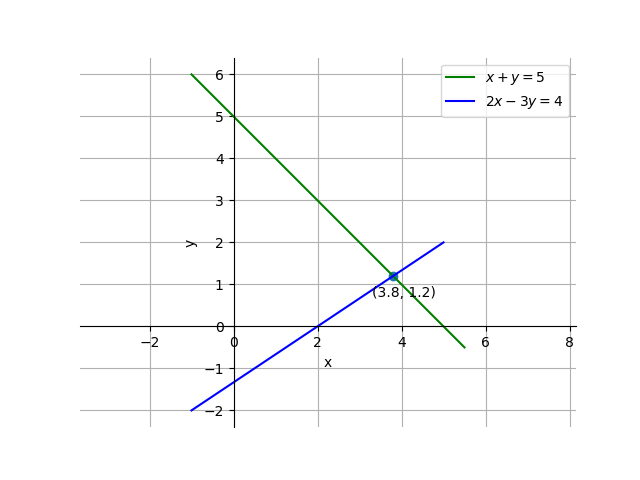
\includegraphics[width=\columnwidth, height=0.8\textheight, keepaspectratio]{Figs/plot(py+C).png}     
\end{frame}

%-------End of Python+C-------------


\begin{frame}[fragile]
    \frametitle{Python Code}
    \begin{lstlisting}
import numpy as np
import matplotlib.pyplot as plt
import numpy.linalg as LA


M = np.array([[1, 1],
              [2,-3]])
b = np.array([5,4])
x = LA.solve(M, b)


plt.scatter(x[0],x[1])


\end{lstlisting}
\end{frame}

\begin{frame}[fragile]
    \frametitle{Python Code}
    \begin{lstlisting}

plt.plot([-1,5.5], [6,-0.5], c='red', label = '$x+y=5$')
plt.plot([-1,5], [-2,2], c='blue', label = '$2x-3y=4$')

plt.annotate(
        f'{x[0],x[1]}',
        xy=(x[0],x[1]),
        xytext = (-15,-15),
        textcoords = "offset points"
        )

\end{lstlisting}
\end{frame}

\begin{frame}[fragile]
    \frametitle{Python Code}
    \begin{lstlisting}

ax = plt.gca()
ax.spines['top'].set_color('none')
ax.spines['bottom'].set_position('zero')
ax.spines['right'].set_color('none')
ax.spines['left'].set_position('zero')
plt.xlabel('x')
plt.ylabel('y')
plt.legend(loc='best')
plt.grid()
plt.axis('equal')

plt.savefig("../Figs/plot(py).png")
plt.show()


    \end{lstlisting}
\end{frame}


\begin{frame}{Plot-Using Python only}
    \centering
    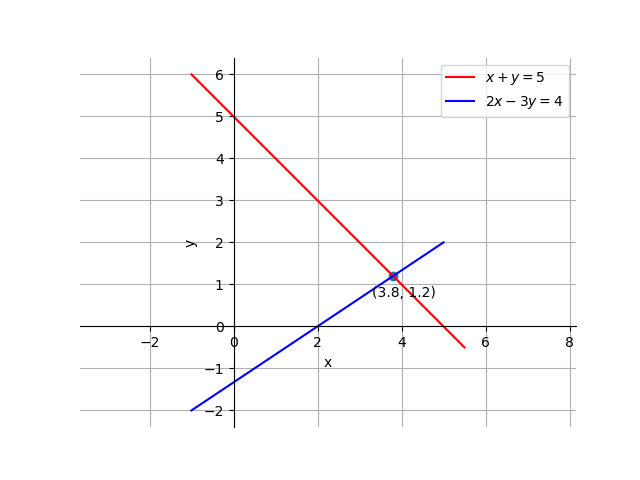
\includegraphics[width=\columnwidth, height=0.8\textheight, keepaspectratio]{Figs/plot(py).png}     
\end{frame}


\end{document}
